\documentclass[]{revdetua}
\usepackage{graphicx}
\usepackage{float}
\usepackage{listings}

\begin{document}

\Header{Volume}{2}{Dezembro}{2022}{0}

\title{Advanced Algorithms Second Project \linebreak Maximum Cut Problem}
\author{Daniela Dias 98039}
\maketitle

\begin{abstract}
This report showcases algorithmic solutions for the Maximum Cut Problem, including a formal analysis of each algorithm's efficiency, a discussion of the obtained results, and predictions for large problem instances. This problem is addressed by the course "Advanced Algorithms" at the University of Aveiro. The proposed algorithms include two randomized algorithms, Las Vegas algorithm and Monte Carlo algorithm. The chosen coding language was Python(3.10).
\end{abstract}

\begin{resumo}
Este relatório apresenta soluções algorítmicas para o problema Maximum Cut, incluindo uma análise formal da eficência de cada algoritmo, uma discussão dos resultados obtidos e previsões para problemas de maior escala. Este problema é abordado pelo curso "Algoritmos Avançados" na Univerdade de Aveiro. Os algoritmos propostos incluem dois algoritmos probabilísticos, algoritmo Las Vegas e algoritmo Monte Carlo. A linguagem de programação escolhida foi o Python(3.10).
\end{resumo}

\begin{keywords}% Note: in English (optional)
Graph, Cut, Cut Set, Maximum Cut, Vertices, Edges, Las Vegas Algorithm, Monte Carlo Algorithm
\end{keywords}

\begin{palavraschave}% Note: in Portuguese (optional)
Grafo, Cut, Cut Set, Maximum Cut, Vértices, Arestas, Algoritmo Las Vegas, Algoritmo Monte Carlo
\end{palavraschave}

\section{Introduction}
This report addresses the second project of "Advanced Algorithms". For this project, we design and test two randomized algorithms to solve the Maximum Cut problem, Las Vegas algorithm and Monte Carlo algorithm.

The following sections describe the problem in detail, explain the added optimizations (in particular, with handling graphs), and analyze the computational complexity of the developed algorithms. For this analysis, we perform a formal and experimental computational complexity analysis of the algorithms. The latter includes a series of experiments for progressively larger problem instances to register and study the number of basic operations carried out, the number of solutions tested, and the execution time. Finally, we compare the results of both the formal and experimental analyses.

We submitted the code files and the results files from the execution of all algorithms. To run the code, first generate the graphs, then run the chosen algorithm file:

\begin{verbatim}
$ python generate_graphs.py 
$ python las_vegas_algorithm.py
$ python monte_carlo_algorithm.py
\end{verbatim}

\section{Maximum Cut Problem}

This report handles the Maximum Cut Problem, which we can solve by finding the maximum cut for a given undirected graph G(V, E), with n vertices and m edges. In graph theory, a cut is a partition of the vertices of a graph into two disjoint subsets, determining a set of edges with one endpoint in each subset. These edges are said to cross the cut. A maximum cut of G is a partition of the graph's vertices into two complementary subsets S and T, such that the number of edges between the set S and the set T is as large as possible [1]. 

In the context of the problem, it's relevant to evaluate the characteristics of the graphs and their structure. The graph instances used in the computational experiments represent the following scenario:
\begin{itemize}
\item Graph vertices are 2D points on the XoY plane, with integer-valued coordinates between 1 and 20.
\item Graph vertices should neither be coincident nor too close.
\item The number of edges sharing a vertex is randomly determined.
\item Use 12.5\%, 25\%, 50\%, and 75\% of the maximum number of edges for the number of vertices.
\item Graph edges are unweighted and undirected.
\end{itemize}

Since the number of edges can be significantly smaller than the number of vertices (when generating the graph instances, we use 12.5\% and 25\% of the maximum number of edges for the number of vertices), we can confirm that the generated graphs aren't all connected. A connected graph is a graph linked in the sense of a topological space: there is a path from any point to any other point in the graph (an edge connecting all vertices). A graph that is not connected is said to be disconnected.

This matters to our problem for the following reasons:
\begin{itemize}
\item The cut set must result in a partition of the vertices into two non-empty disjoint subsets.
\item Vertices without edges have zero impact in a cut set (the number of edges crossing the cut doesn't change).
\end{itemize}

Hence, we were able to implement optimizations that restricted the problem to a smaller version (subset) of the problem. Instead of working with the complete graph, we work with a subgraph of the initial graph, ignoring vertices without edges (with a degree equal to zero). This optimization decreases the computational complexity of the problem.

The first step to constructing a graph is generating the list of vertices and edges. The list of vertices is a list of randomly generated tuples of coordinates with 2, 4, 8, 16, 32, 62, 128, and 256 vertices (numbers by the power of 2). The coordinates take values between 1 and 20, inclusive. Since the graph is undirected in this context, the list of edges is a list of the tuples of the vertices involved  (their coordinates). Consequently, (x1, x2) is the equivalent of (x2, x1). Following are the examples of generated vertices and edges:

\begin{itemize}
\item Vertices: [(5, 3), (12, 15), (11, 19), (3, 17)]
\item Edges: [((3, 17), (11, 19)), ((12, 15), (3, 17)), ((5, 3), (3, 17)), ((12, 15), (5, 3))]
\end{itemize}

To enable the storage of graphs (in JSON files), we chose to identify the vertices by numeric id's and convert the graphs data in a node-link format suitable for JSON serialization and use in Javascript documents, with networkx.node\_link\_data(graph). An example, with the previous vertices and edges, would be:

\begin{itemize}
\item {"directed": false, "multigraph": false, "graph": {}, "nodes": [{"id": 0}, {"id": 1}, {"id": 2}, {"id": 3}], "links": [{"source": 0, "target": 3}, {"source": 0, "target": 1}, {"source": 1, "target": 3}, {"source": 2, "target": 3}]}
\end{itemize}

To load the graph files, we have to read the file and convert the read data with nx.node\_link\_graph(graph\_data). Finally, we identify each cut set by the vertices partition, A and B. For example:

\begin{itemize}
\item A:  [3]
\item B:  [0, 1, 2]
\end{itemize}

\section{Analysis of Algorithm Efficiency}

\subsection{Measuring an Input’s Size}

It is logical to investigate an algorithm’s efficiency as a function of some parameter n indicating the algorithm’s input size. For this case, n could be the size of the list of vertices in the generated graphs. However, since the algorithm only examines the connected vertices (with at least one edge), we measured the input size by the number of connected vertices.

\subsection{Units for Measuring Running Time}

For measuring the running time of the algorithms developed, we decided to use two units of time measurement: execution time in seconds and the number of basic operations executed by the algorithm. 

It is worth noting that the first measurement has drawbacks since it depends on the speed of the computer running the program, the implementation of the algorithm, and the compiler used in generating the machine code. On the other hand, we can objectively measure the running time by identifying a basic operation and computing the number of times this operation is executed on inputs of size n. 

The basic operation contributes the most to the total running time: it is the most time-consuming operation in the algorithm's innermost loop. In our case, since we have adapted the code from the first project to have more control over the creation of subsets (generation of solutions to be tested), we can and should consider the generation of random vertices as the basic operation. It is the most time-expensive block of code, in particular, with the creation of repeated vertices and subsets. This adaptation was made possible by replacing the imported function, itertools.combinations(), with the creation and addition of random vertices to a subset with the function np.random.randint().

The creation of subset B is relatively fast: we obtain the difference between the set of total vertices and the random subset, meaning the order of growth is constant. Therefore, we don't include it in our calculations. 

\subsection{Worst-Case, Best-Case, and Average-Case Efficiencies}

We have established that it is reasonable to measure an algorithm’s efficiency as a function of the size of the algorithm’s input. However, the running time of the same algorithm can be quite different for the same list size n. Hence, we will consider the worst-case and best-case efficiencies when analyzing the developed algorithms.

The worst-case efficiency of an algorithm is its efficiency for the worst-case input of size n (for which the algorithm runs the longest among all possible inputs of that size). For our algorithms, the worst-case happens for the largest number of generated vertices/subsets (with repetition) among all possible inputs of size n. This analysis provides important information about an algorithm’s efficiency by bounding its running time from above. 

The best-case efficiency of an algorithm is its efficiency for the best-case input of size n (for which the algorithm runs the fastest among all possible inputs of that size). For our algorithms, the best-case happens for the smallest number of generated vertices/subsets among all possible inputs of size n, in other words, when we find the best solution in the first iteration.

Finally, the average-case of an algorithm is its efficiency for the "typical" (or random) case input of size n. It is the most challenging to calculate.

\section{Randomized Algorithms}

A randomized algorithm incorporates a certain amount of randomness into its logic or process. To achieve good performance in the "average case", this type of algorithm typically uses uniformly random bits as an auxiliary input to direct its behavior. As a result, either the running time or the output (or both) are random variables. It's also worth noting that, instead of using a real source of random bits, pseudorandom number generators are used to approximate randomized algorithms [3].

For randomized algorithms, there is, at least theoretically, a single correct solution for a given problem. The probabilistic aspects, however, differ from one execution of the algorithm to the next:

\begin{itemize}
\item Whether the solution is found or not.
\item The precision of the solution.
\item The time it takes to reach the solution. 
\end{itemize}

There are two major categories of randomized algorithms, which we will be covering in this report: Monte Carlo and Las Vegas. Monte Carlo algorithms are always computationally fast, yet they only return the correct answer with a given probability. Las Vegas algorithms always deliver the solution, yet they are not guaranteed to meet our shorter time expectations.

We can convert Las Vegas algorithms into a Monte Carlo algorithm by having it output a possibly incorrect answer if it fails to complete within a predetermined time or number of operations. On the other hand, we can change a Monte Carlo algorithm into a Las Vegas algorithm by removing any parameters that bound the running time [3]. We applied this to the development of our algorithms.

For both algorithms, we iterate through the randomly generated candidate solutions and keep the best feasible solution computed. We also keep track of tested solutions/configurations so that we do not consider solutions more than once. Finally, we stop testing candidate solutions when we obtain a maximum cut set with a value equal to the total number of edges in the graph (representing the best theoretical solution possible). However, this last optimization experimentally only improved the computational complexity of problem instances with fewer vertices and edges ($\leq$ 4 vertices and $\leq$ 4 edges).

We attempted multiple implementations for obtaining a random subset  (and, consequently, a partition of vertices):

A first implementation decided on a random size between 0 and the number of vertices and generated subsets with that given size (returning a python generator). Then, by iterating through the subsets and randomly generating a number between 0 and 1 in each iteration, we decided whether the current subset was chosen (0 - Not chosen, 1 - Chosen). However, this implementation meant that the first subsets (from the combinations generated) had a higher probability of being tested. Despite producing very accurate results in a short execution time for the Monte Carlo algorithm, we had to discard this approach and replace it with another implementation to ensure the algorithm's randomness.

\pagebreak

\begin{verbatim}
# Generate subsets with random size
size = np.random.randint(0, len(vertices) + 1)

for subset in combinations(vertices, size):
    if np.random.randint(0, 2):
        break
\end{verbatim}

For a second implementation, we also randomly decided on a size between 0 and the number of vertices, and we generated subsets with that size (returning a python generator). Before proceeding, we calculated the total number of subsets generated with the received size, in order to obtain a random index: a random number between 0 and the current number of subsets. Then, the algorithm iterated through all the subsets and stopped once the subset index matched the random index, giving us the desired subset. 

This approach solved the problem faced with the first assignment of ”Advanced Algorithms”, in particular, with the Exhaustive Search algorithm. Due to a lack of memory, the algorithm failed to provide the solution for graphs with more than 16 vertices. However, this second algorithm didn't address all issues, since the number of subsets with larger problem instances was out of bounds for int64 (randint limitations).

\begin{verbatim}
# Generate subsets with random size
size = np.random.randint(0, len(vertices) + 1)

# Get random subset
n_subsets = math.comb(len(vertices), size)
random_index = np.random.randint(0, n_subsets, 
                            dtype=np.int64)

subset_idx = 0
for subset in combinations(vertices, size):
    if subset_idx == random_index:
        break

    subset_idx += 1
\end{verbatim}

The final implementation took into consideration the previously mentioned issues. Instead of generating all the subsets with a given size, we:
\begin{itemize}
\item Randomly decide a size between 0 and the number of vertices.
\item Generate and add random vertices to the current subset until that subset has the desired size. 
\end{itemize}

This algorithmic solution proved to be highly efficient by only generating the random subset. It avoided the need for spending computational power, time, and memory on creating many unnecessary subsets (for an asked size).

\pagebreak

\begin{verbatim}
# Generate subsets with random size
size = np.random.randint(0, len(vertices)+1)

# Generate subset with random vertices
subset = []
while len(subset) != size:
    random_index = np.random.randint(0, 
                        len(vertices))
    if vertices[random_index] not in subset:
        subset.append(vertices[random_index])
\end{verbatim}

\section{Las Vegas Algorithm}

Las Vegas algorithms are guaranteed to give the correct answer in all the cases, but their execution time is probabilistic. Thus, even though they are generally expected to be fast, and will always return the correct answer, it can happen (with a relatively low probability) that they take a long time to answer.

The nature of Las Vegas algorithms makes them suitable in situations where the number of possible solutions is limited and verifying the correctness of a candidate solution is relatively easy [4]. For our problem, the algorithm failed to give a solution within an acceptable time for graphs with more than 16 vertices. Hence, we discarded these graphs for the experimental analysis. 

As mentioned previously, we consider the basic operation to be the generation of a single random vertex (along with its addition to the current subset). Since we include the optimization of stopping testing solutions once we find the best solution possible, the algorithm will only test one subset in the best case. On the other hand, trying one solution is equivalent to having a number of basic operations equal to the number of vertices inside the subset, which, in the best scenario, will be a single generated vertex. Hence, the best case is constant: $\Omega(n)$ = 1.

In the worst case, the algorithm won't find the best solution mid-simulation and will generate repeated random vertices and subsets until it has considered all possible solutions. This repetition makes it difficult to predict the number of basic operations for n (the total number of vertices with edges). However, being \(2^n\) the number of all different configurations to be tested, we know that the number of basic operations will be equal to \(2^n\) multiplied by a constant value. This value depends on the amount of "luck" throughout the simulation, being smaller for less repeated vertices/subsets. 

With this, we can conclude that the order of growth is exponential: $O(n)$ = \(C 2^n\) = \(2^n\). The algorithm is simple but costly in both time and space complexity, and larger problem instances will result in a quickly rising number of iterations.

\section{Monte Carlo Algorithm}

Although Monte Carlo algorithms are computationally faster, they may or not find the solution: there is a probability of finding the correct answer that can be computed and controlled through the algorithm parameters. The error probability can be low, even within efficient execution time. Meanwhile, the execution time for these algorithms is deterministic.

To study the probability of finding the correct answer for different deterministic running times, we tried the following algorithm parameters:

\begin{itemize}
\item Operations: 100000 - Time Limit: None.
\item Operations: 1000000 - Time Limit: None.
\item Operations: None - Time Limit: 60s.
\item Operations: None - Time Limit: 120s.
\item Operations: 5000000 - Time Limit: 120s.
\end{itemize}

If the number of operations exceeds the provided operations limit, we decide to stop testing altogether. The same applies when the algorithm exceeds the time limit.

\section{Results}

\subsection{Maximum Cut}

As mentioned, the Las Vegas algorithm is guaranteed to give the correct answer for all problem instances (we consider it for graphs solvable within an acceptable running time). In terms of accuracy, this algorithm is equivalent to the Exhaustive Search algorithm developed in the first project. For any problem with 16 or fewer vertices, both promise 100\% accuracy for calculating the maximum cut. These results are relevant for analyzing the solutions obtained from the execution of other algorithms, at least until 16 vertices. 

\begin{table}[!ht]
    \centering
    Las Vegas Algorithm
    \begin{tabular}{|l|l|l|l|}
    \hline
        Graph & Vertices & Edges & Maximum\_Cut \\ \hline
        4 & 2 & 1 & 1 \\ \hline
        4 & 4 & 3 & 3 \\ \hline
        4 & 4 & 4 & 3 \\ \hline
        8 & 6 & 3 & 3 \\ \hline
        8 & 7 & 7 & 6 \\ \hline
        8 & 8 & 14 & 11 \\ \hline
        8 & 8 & 21 & 15 \\ \hline
        16 & 15 & 15 & 13 \\ \hline
        16 & 16 & 30 & 23 \\ \hline
        16 & 16 & 60 & 41 \\ \hline
        16 & 16 & 90 & 56 \\ \hline
    \end{tabular}
\end{table}

\begin{table}[!ht]
    \centering
    Exhaustive Algorithm
    \begin{tabular}{|l|l|l|l|}
    \hline
        Graph         & Vertices      & Edges       & Maximum Cut      \\ \hline
        4 & 2 & 1 & 1 \\ \hline
        4 & 4 & 3 & 3 \\ \hline
        4 & 4 & 4 & 3 \\ \hline
        8 & 6 & 3 & 3 \\ \hline
        8 & 7 & 7 & 6 \\ \hline
        8 & 8 & 14 & 11 \\ \hline
        8 & 8 & 21 & 15 \\ \hline
        16 & 15 & 15 & 13 \\ \hline
        16 & 16 & 30 & 23 \\ \hline
        16 & 16 & 60 & 41 \\ \hline
        16 & 16 & 90 & 56 \\ \hline
    \end{tabular}
\end{table}

\pagebreak

For the first implementation of the Monte Carlo algorithm, with a 100000 operations limit, 64\% of the results were correct, failing only for the last graphs with 16 vertices (where the number of needed operations exceeded the limit). With this restriction, the number of solutions tested experimentally did not surpass 4300. 

\begin{table}[!ht]
    \centering
    Monte Carlo Algorithm with 100000 operations limit
    \begin{tabular}{|l|l|l|l|}
    \hline
        Graph & Vertices & Edges & Maximum Cut \\ \hline
        4 & 2 & 1 & 1 \\ \hline
        4 & 4 & 3 & 3 \\ \hline
        4 & 4 & 4 & 3 \\ \hline
        8 & 6 & 3 & 3 \\ \hline
        8 & 7 & 7 & 6 \\ \hline
        8 & 8 & 14 & 11 \\ \hline
        8 & 8 & 21 & 15 \\ \hline
        16 & 15 & 15 & 12 \\ \hline
        16 & 16 & 30 & 22 \\ \hline
        16 & 16 & 60 & 40 \\ \hline
        16 & 16 & 90 & 55 \\ \hline
    \end{tabular}
\end{table}

The second implementation of the Monte Carlo algorithm, with a 1000000 operations limit, had a 100\% accuracy. As expected, by setting up a higher operations limit, the number of solutions tested increased, and, therefore, the accuracy improved (with the cost of a higher running time). However, the accuracy could have been lower than observed as, for graphs with 16 vertices and more, the algorithm hit the maximum number of operations allowed (meaning it did not test all solutions). Experimentally, the algorithm managed to test up to 27295 different solutions max.

\begin{table}[!ht]
    \centering
    Monte Carlo Algorithm with 1000000 operations limit
    \begin{tabular}{|l|l|l|l|}
    \hline
        Graph & Vertices & Edges & Maximum Cut \\ \hline
        4 & 2 & 1 & 1 \\ \hline
        4 & 4 & 3 & 3 \\ \hline
        4 & 4 & 4 & 3 \\ \hline
        8 & 6 & 3 & 3 \\ \hline
        8 & 7 & 7 & 6 \\ \hline
        8 & 8 & 14 & 11 \\ \hline
        8 & 8 & 21 & 15 \\ \hline
        16 & 15 & 15 & 13 \\ \hline
        16 & 16 & 30 & 23 \\ \hline
        16 & 16 & 60 & 41 \\ \hline
        16 & 16 & 90 & 56 \\ \hline
    \end{tabular}
\end{table}

The third implementation of the Monte Carlo algorithm, with a 60 seconds limit, had a 100\% accuracy. However, we also did not test all solutions for graphs with 16 vertices, meaning that 100\% accuracy isn't guaranteed. On the other hand, this version is statistically more accurate than the previous ones, overall testing more solutions (experimentally, the maximum was 67004 different solutions).

\begin{table}[!ht]
    \centering
    Monte Carlo Algorithm with 60 seconds limit
    \begin{tabular}{|l|l|l|l|}
    \hline
        Graph & Vertices & Edges & Maximum Cut \\ \hline
        4 & 2 & 1 & 1 \\ \hline
        4 & 4 & 3 & 3 \\ \hline
        4 & 4 & 4 & 3 \\ \hline
        8 & 6 & 3 & 3 \\ \hline
        8 & 7 & 7 & 6 \\ \hline
        8 & 8 & 14 & 11 \\ \hline
        8 & 8 & 21 & 15 \\ \hline
        16 & 15 & 15 & 13 \\ \hline
        16 & 16 & 30 & 23 \\ \hline
        16 & 16 & 60 & 41 \\ \hline
        16 & 16 & 90 & 56 \\ \hline
    \end{tabular}
\end{table}

For the fourth implementation, with 120 seconds, the empirical accuracy was 100\%. Once again, the algorithm returned the maximum cut without testing all combinations for graphs with 16 vertices, meaning the accuracy can decline with more simulations. However, this version is expected to be more accurate than the others, with more configurations tested (attempts) on average. The maximum number of different solutions was 86508.

\begin{table}[!ht]
    \centering
    Monte Carlo Algorithm with 120 seconds limit
    \begin{tabular}{|l|l|l|l|}
    \hline
        Graph & Vertices & Edges & Maximum Cut \\ \hline
        4 & 2 & 1 & 1 \\ \hline
        4 & 4 & 3 & 3 \\ \hline
        4 & 4 & 4 & 3 \\ \hline
        8 & 6 & 3 & 3 \\ \hline
        8 & 7 & 7 & 6 \\ \hline
        8 & 8 & 14 & 11 \\ \hline
        8 & 8 & 21 & 15 \\ \hline
        16 & 15 & 15 & 13 \\ \hline
        16 & 16 & 30 & 23 \\ \hline
        16 & 16 & 60 & 41 \\ \hline
        16 & 16 & 90 & 56 \\ \hline
    \end{tabular}
\end{table}

The final implementation, with a 120 seconds limit and 5000000 operations limit, failed to deliver any additional conclusions. The results were very similar to the other versions of the Monte Carlo algorithm, in particular with a 120 seconds limit. The accuracy was also 100\%, while sometimes hitting the operation limit before the time limit. 

\begin{table}[!ht]
    \centering
    Monte Carlo Algorithm with 120 seconds limit  and 5000000 operations limit
    \begin{tabular}{|l|l|l|l|}
    \hline
        Graph & Vertices & Edges & Maximum Cut \\ \hline
        4 & 2 & 1 & 1 \\ \hline
        4 & 4 & 3 & 3 \\ \hline
        4 & 4 & 4 & 3 \\ \hline
        8 & 6 & 3 & 3 \\ \hline
        8 & 7 & 7 & 6 \\ \hline
        8 & 8 & 14 & 11 \\ \hline
        8 & 8 & 21 & 15 \\ \hline
        16 & 15 & 15 & 13 \\ \hline
        16 & 16 & 30 & 23 \\ \hline
        16 & 16 & 60 & 41 \\ \hline
        16 & 16 & 90 & 56 \\ \hline
    \end{tabular}
\end{table}

\pagebreak

For larger problem instances, we're unable to objectively measure the accuracy of the multiple versions of the Monte Carlo algorithm. However, we can assume that it is (programmatically) impossible for the algorithm to return a cut larger than the correct maximum cut: it returns a smaller cut value if it fails to return the expected solution. Taking this into consideration, we can compare the different implementations of the Monte Carlo algorithm to confirm which returns the highest maximum cut, in other words, the most accurate result.

For the graphs with at least 16 vertices, the Monte Carlo algorithm obtained:
\begin{itemize}
\item With a 100000 operations limit, \textbf{0} of the greatest cut sets.
\item With a 1000000 operations limit, \textbf{4} of the greatest cut sets. 
\item With a 60 seconds time limit,  \textbf{4} of the greatest cut sets. 
\item With a 120 seconds time limit,  \textbf{5} of the greatest cut sets. 
\item With a 5000000 operations limit and a 120 seconds time limit, \textbf{6} of the greatest cut sets.
\end{itemize}

\begin{table}[!ht]
    \centering
    Greatest Maximum Cuts obtained by the different Monte Carlo algorithm versions
    \begin{tabular}{|l|l|l|l|l|l|}
    \hline
        V0 & V1 & V2 & V3 & V4 & Max \\ \hline
        44 & 45 & 45 & 45 & 47 & 47 \\ \hline
        78 & 83 & 83 & 83 & 85 & 85 \\ \hline
        141 & 153 & 146 & 149 & 150 & 153 \\ \hline
        205 & 206 & 209 & 211 & 208 & 211 \\ \hline
        151 & 157 & 155 & 155 & 157 & 157 \\ \hline
        280 & 296 & 293 & 293 & 291 & 296 \\ \hline
        540 & 553 & 554 & 554 & 550 & 554 \\ \hline
        790 & 802 & 806 & 801 & 801 & 806 \\ \hline
        546 & 559 & 560 & 560 & 563 & 563 \\ \hline
        1057 & 1083 & 1094 & 1097 & 1090 & 1097 \\ \hline
        2085 & 2105 & 2128 & 2127 & 2121 & 2128 \\ \hline
        3128 & 3134 & 3140 & 3140 & 3143 & 3143 \\ \hline
        2117 & 2173 & 2128 & 2134 & 2173 & 2173 \\ \hline
        4174 & 4188 & 4233 & 4227 & 4202 & 4233 \\ \hline
        8277 & 8324 & 8342 & 8360 & 8331 & 8360 \\ \hline
        12345 & 12370 & 12416 & 12424 & 12419 & 12424 \\ \hline
    \end{tabular}
\end{table}

It is also relevant to analyze the obtained solutions by comparing them with the algorithms of the first project. As stated in the first report, the Local Search algorithm (the first greedy algorithm) was significantly less correct than the Breadth-First search, obtaining a maximum cut considerably lower than the intended. Hence, we don't consider it for this analysis. 

For graphs up to 16 vertices, 36\% of the results obtained by the Breadth-First algorithm matched the correct maximum cut. All versions of the Monte Carlo algorithm returned better results compared to this algorithm ($\geq$ 64\%). For graphs with more than 16 vertices, the Breadth-First search behaved similarly to the first version of the Monte Carlo algorithm (the least accurate version), returning only a greater maximum cut for the graph with 256 vertices and 8160 edges.

\begin{table}[!ht]
    \centering
    Breadth-First Search and Monte Carlo Algorithm Comparison (Maximum Cut)
    \begin{tabular}{|l|l|l|l|}
    \hline
        Vertices & Edges & Breadth-First & Monte Carlo V0 \\ \hline
        32 & 62 & 33 & 44 \\ \hline
        32 & 124 & 67 & 78 \\ \hline
        32 & 248 & 131 & 141 \\ \hline
        32 & 372 & 163 & 205 \\ \hline
        64 & 252 & 142 & 151 \\ \hline
        64 & 504 & 250 & 280 \\ \hline
        64 & 1008 & 446 & 540 \\ \hline
        64 & 1512 & 508 & 790 \\ \hline
        128 & 1016 & 517 & 546 \\ \hline
        128 & 2032 & 1015 & 1057 \\ \hline
        128 & 4064 & 1824 & 2085 \\ \hline
        128 & 6096 & 2315 & 3128 \\ \hline
        256 & 4080 & 2070 & 2117 \\ \hline
        256 & 8160 & 4199 & 4174 \\ \hline
        256 & 16320 & 7669 & 8277 \\ \hline
        256 & 24480 & 8206 & 12345 \\ \hline
    \end{tabular}
\end{table}

\subsection{Basic Operations}

\begin{figure}[H]
    \centering
    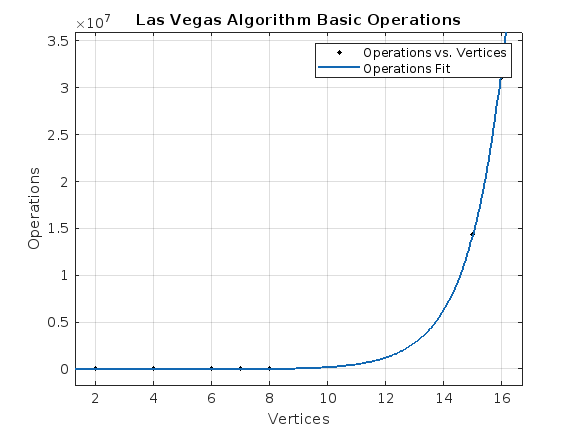
\includegraphics[width=9cm]{Las Vegas Algorithm/Las Vegas Algorithm Basic Operations.png}
    \caption{Exhaustive Search Basic Operations}
\end{figure}

By fitting the data to a general model Exponential, we achieve:
\begin{verbatim}
     f(x) = a*exp(b*x)
Coefficients (with 95% confidence bounds):
       a =       68.28  (-64.1, 200.7)
       b =      0.8173  (0.6956, 0.9389)

Goodness of fit:
  SSE: 5.07e+12
  R-square: 0.9978
  Adjusted R-square: 0.9975
  RMSE: 7.506e+05
\end{verbatim}

\pagebreak
  
This model is useful for calculating the computational complexity of larger problem instances. Also, as we can evaluate from the previous graph, the empirical analysis matches what was stated in the formal analysis:
\begin{itemize}
\item The Las Vegas algorithm's order of growth is exponential.
\end{itemize}


\subsection{Solutions Tested}

\begin{figure}[H]
    \centering
    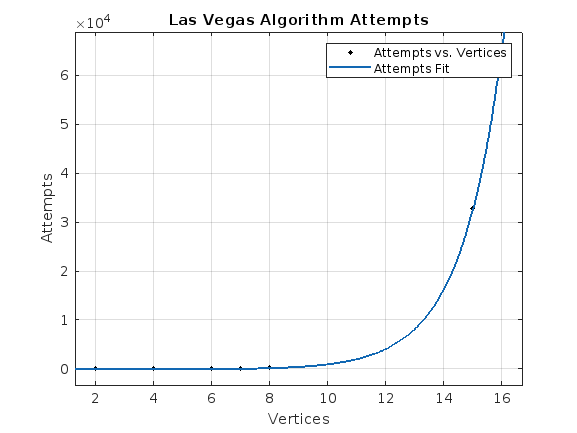
\includegraphics[width=9cm]{Las Vegas Algorithm/Las Vegas Algorithm Attempts.png}
    \caption{Exhaustive Search Basic Operations}
\end{figure}

By fitting the data to a general model Exponential, we achieve:
\begin{verbatim}
     f(x) = a*exp(b*x)
Coefficients (with 95% confidence bounds):
       a =      0.9994  (0.9761, 1.023)
       b =      0.6932  (0.6917, 0.6947)

Goodness of fit:
  SSE: 3769
  R-square: 1
  Adjusted R-square: 1
  RMSE: 20.47
\end{verbatim}
  
Although the Las Vegas algorithm and the Exhaustive Search algorithm differ in implementation, they both apply the same principle: test all possible configurations (or solutions). However, for this second project, we added the following optimization:

\begin{itemize}
\item Stop testing candidate solutions when we obtain the best theoretically possible solution - a maximum cut set with a value equal to the total number of edges in the graph.
\end{itemize}

This added optimization explains the difference observed in the number of attempts for each of the two algorithms. 

As stated in the previous project, the generation of all possible combinations creates \(2^n\) partitions (n being the number of vertices with edges). While the Exhaustive Search algorithm tries exactly \(2^n\) configurations, the Las Vegas algorithm tries \(2^n\) or fewer configurations if the best solution is obtained mid-simulation. We notice this with graphs with $\leq$ 4 vertices and $\leq$ 4 edges. Without the optimization, the number of solutions tested would be the same for both algorithms.

\begin{table}[!ht]
    \centering
    Exhaustive Search Algorithm and Las Vegas Algorithm Comparison (Solutions Tested)
    \begin{tabular}{|l|l|l|}
    \hline
        Vertices & Exhaustive Search & Las Vegas Algorithm \\ \hline
        2 & 4 & 3 \\ \hline
        4 & 16 & 9 \\ \hline
        4 & 16 & 16 \\ \hline
        6 & 64 & 3 \\ \hline
        7 & 128 & 128 \\ \hline
        8 & 256 & 256 \\ \hline
        8 & 256 & 256 \\ \hline
        15 & 32768 & 32768 \\ \hline
        16 & 65536 & 65536 \\ \hline
        16 & 65536 & 65536 \\ \hline
        16 & 65536 & 65536 \\ \hline
    \end{tabular}
\end{table}

\subsection{Execution Time}

Finally, we proved that the execution time (in seconds) is not a good measurement of running time, as it produces different results for the same input of size n and for the same number of executed operations.

\begin{figure}[H]
    \centering
    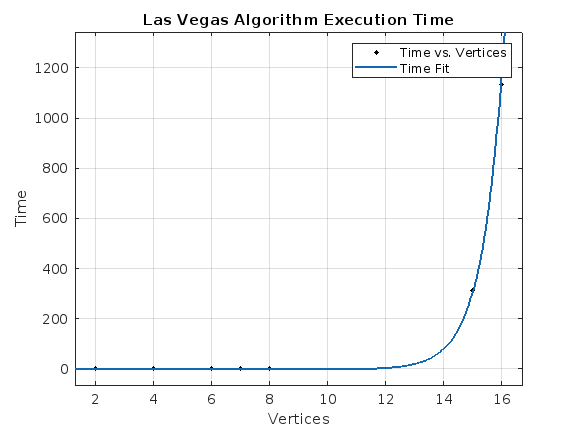
\includegraphics[width=9cm]{Las Vegas Algorithm/Las Vegas Algorithm Execution Time.png}
    \caption{Exhaustive Search Basic Operations}
\end{figure}

By fitting the data to a general model Exponential, we achieve:
\begin{verbatim}
     f(x) = a*exp(b*x)
Coefficients (with 95% confidence bounds):
       a =   5.401e-07  (-1.658e-06, 2.738e-06)
       b =       1.345  (1.09, 1.6)

Goodness of fit:
  SSE: 1.088e+04
  R-square: 0.9964
  Adjusted R-square: 0.996
  RMSE: 34.77
\end{verbatim}

However, at the same time, this model is useful for calculating the computational complexity of larger problem instances and, once again, the empirical analysis matches what was stated in the formal analysis:
\begin{itemize}
\item The Las Vegas algorithm's order of growth is exponential.
\end{itemize}

\subsection{Larger Problem Instances}

Finally, we can estimate the execution time for much larger problem instances with the general models we computed for the number of basic operations and the running time.

For graphs with n = 32 vertices (with edges), the number of basic operations will be  \(68.28\:\cdot \:e^{0.8173\cdot \:32} =1.55832\dots E13\) and the execution time \(5.401\cdot 10^{-7}\cdot \:e^{1.345\cdot 32} = 2657716657505\) seconds.

For graphs with n = 64 vertices (with edges), the number of basic operations will be \(68.28\:\cdot \:e^{0.8173\cdot \:64} = 3.55649\dots E24 \) and the running time \(5.401\cdot 10^{-7}\cdot \:e^{1.345\cdot 64} = 1.30781\dots E31\) seconds.

\section{Conclusion}

To conclude this document, we now understand the advantages and disadvantages of randomized algorithms. Randomized algorithms are known for their simplicity and efficiency, requiring little execution time and memory space compared to deterministic algorithms. However, implementation decisions matter, as the addition of restrictions (which limit the number of tested configurations) can lower the algorithm's reliability by not finding the right solution.

At the same time, the quality of these algorithms depends on the quality of the random number generator used as part of the algorithm. As once stated, we use pseudorandom number generators to approximate the randomized algorithms, which bring up, for example, the following problems [5]: 

\begin{itemize}
\item Lack of uniform distribution for large quantities of generated numbers.
\item Correlation of successive values.
\item Poor dimensional distribution of the output.
\end{itemize}

Finally, for evaluating randomized algorithms, it's worth noting that the probabilistic aspects differ from one execution of the algorithm to the next, especially with the Monte Carlo algorithms that don't guarantee the correct solution.

\begin{thebibliography}{00}

\bibitem{b1} Wikipedia (2022). \textit{Maximum cut} [Online]. Available: \url{https://en.wikipedia.org/wiki/Maximum_cut}
\bibitem{b2} Shiva Basava P. \textit{Maximum cut Problem} [Online]. Available: \url{https://iq.opengenus.org/maximum-cut-problem}
\bibitem{b3} Wikipedia (2022). \textit{Randomized Algorithm} [Online]. Available: \url{https://en.wikipedia.org/wiki/Randomized_algorithm}
\bibitem{b4} Wikipedia (2022). \textit{Las Vegas Algorithm} [Online]. Available: \url{https://en.wikipedia.org/wiki/Las_Vegas_algorithm}
\bibitem{b5} Wikipedia (2022). \textit{Pseudorandom number generator} [Online]. Available: \url{https://en.wikipedia.org/wiki/Pseudorandom_number_generator}

\end{thebibliography}

\end{document}
